\begin{frame}
	\frametitle{Grover's algorithm: Outline}
	\begin{tikzpicture}[
	expl/.style={draw=black, thick=2pt,fill=blue!20,rounded corners},
	arrow/.style={red!80!black,ultra thick,->,>=latex}]	
	\node[anchor=south west,inner sep=0] (image) at (0,0) {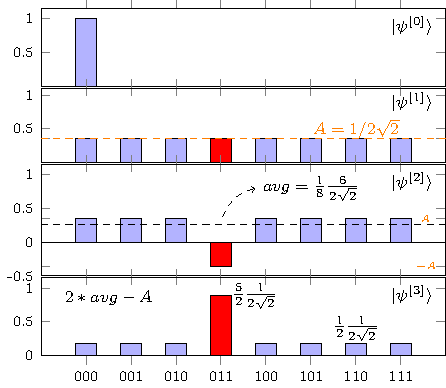
\includegraphics[width=0.5\textwidth]{figures/bar-graph/probs.pdf}};
	\begin{scope}[x={(image.south east)},y={(image.north west)}]
		%\draw[help lines,xstep=.1,ystep=.1] (0,0) grid (1,1);
		%\foreach \x in {0,1,...,9} { \node [anchor=north] at (\x/10,0) {0.\x}; }
		%\foreach \y in {0,1,...,9} { \node [anchor=east] at (0,\y/10) {0.\y}; }
		\node[expl](A) at (1.5,0.875) {\Large Initial state $\ket{\psi^{[0]}}$};
		\node[expl](B) at (1.5,0.65) {\Large Initialization $\ket{\psi^{[1]}}$};
		\node[expl](C) at (1.5,0.4) {\Large Sign flip $\ket{\psi^{[2]}}$};
		\node[expl](D) at (1.5,0.15) {\Large Inversion about average $\ket{\psi^{[3]}}$};
		
		\draw[arrow] (A.south) -- node [right]{Hadamard $H$} (B.north);
		\draw[arrow] (B.south) -- node [right]{Oracle $U_f$} (C.north);
		\draw[arrow] (C.south) -- node [right]{Difussion $U_d$} (D.north);
		\draw[arrow] (D.north east) to[bend right] node [right]{$\frac{\pi}{4}\sqrt{n}$} (B.east);
	\end{scope}

	\end{tikzpicture}	
\end{frame}